\section{Evaluation}
\label{sec:evaluation}
This section presents our implementation prototype and experiments with a case study of developing a software application for LEGO to evaluate the feasibility and usability of our approach.

\subsection{Implementation}
Our approach is implemented as an extension of the Papyrus modeling tool, which is based on Eclipse.
C++ code is generated from architecture models in UML.
The generated code is executed within POSIX systems.
\begin{comment}
%The usage of C++11 standard threads can be easily integrated in the future.
%For incremental code generation in XSeparation, a model listener based on IncQuery is hooked to the modeling tool to detect model modifications.
The additional constructs added to C++ are engineered in a way that allows programmers to use facilities such as auto-completion of any C++ IDE to write fine-grained code without installing additional tools.
The programmers can stay within their familiar IDE such as Eclipse CDT and Visual Studio.
This is one of our advantages over other approaches which will be discussed in Section \ref{sec:relatedwork}. 

In order to synchronize the modified intermediate code with the model, we apply our synchronization methodological pattern presented in \cite{foster2016}.
Following this pattern, we implemented a synchronizer from code to model.
It contains the following use-cases:

\begin{itemize}[\footnotesize]
	\itemsep0em
	\item \tb{Batch code generation}: generates and overwrites existing intermediate code from model.
	\item \tb{Incremental code generation}: propagates changes from the model to the mediate code.
	\item \tb{Batch reverse engineering}: creates and overwrites any existing model from the intermediate code.
	\item \tb{Incremental reverse engineering}: propagates changes from the intermediate code to the model.
\end{itemize}


The batch code generation and reverse engineering are straightforwardly supported by using the bidirectional traceability between the architecture model and the intermediate code created by XSeparation. 
The implementation of incremental code generation (ICG) and reverse engineering (IRE) is based on management of modifications made in model and code.


\begin{table*}[]
	\scriptsize
	\centering
	\caption{Model change classification and management}
	\label{table:modelchangeclassification}
	\begin{tabular}{|l|p{3cm}|l|p{9.5cm}|}
		\hline
		\multicolumn{2}{|c|}{Element type}                              & \multicolumn{1}{c|}{Modification type} & \multicolumn{1}{c|}{Action}                                                                              \\ \hline
		\multirow{3}{*}{Structure} & Part/Port/Connector                & Add/Remove/Update                      & Regenerate Component structure-prescribed code                                                           \\ \cline{2-4} 
		& Class/Component/Interface          & Add/Remove/Update                      & Create/Remove/Update the corresponding code                                                              \\ \cline{2-4} 
		& Property                           & Add/Remove/Update                      & Create/Remove/Regenerate the corresponding class attribute                                               \\ \hline
		\multirow{4}{*}{Behavior}  & Operation                          & Add/Remove/Update                      & Create/Remove/Regenerate the corresponding method with keeping its method body                           \\ \cline{2-4} 
		& \multirow{3}{*}{UML State Machine} & Create                                 & Generate Behavior-prescribed code and State machine action code                                          \\ \cline{3-4} 
		&                                    & Remove                                 & Remove Behavior-prescribed code and State machine action code from the corresponding component           \\ \cline{3-4} 
		&                                    & Update                                 & Regenerate Behavior-prescribed code and State machine action code with respect to the existing user-code \\
		\hline
	\end{tabular}
\end{table*}

\vskip 0.2cm
\noindent
\tb{Incremental code generation:}
A model listener is developed to detect changes in model.
Table \ref{table:modelchangeclassification} shows our detected modifications and how to propagate these changes to the intermediate code.
%The modifications can be detected by a model listener.
We make a distinction between structural and behavioral modifications, which result in creating/removing/regenerating the corresponding code part.
Although only add/remove/update are detected, the moving of a model element can be combined as a removal following by an addition.  
Some particular modifications requires the corresponding actions to respect and preserve the user code.
For example, if the \ttt{sendDataToFifo} method in Listing \ref{lst:producerinteraction} is renamed to \ttt{sendDataFromProducerToFifo} at the model level, the corresponding action consists of several steps: (1) identify the method, at the code level, associated with the operation, at the model level, using the old name \ttt{sendDataToFifo}, which is recorded by the model listener;
(2) rename the method to \ttt{sendDataFromProducerToFifo} while keeping its parameters and body intact. 

\vskip 0.2cm
\noindent
\tb{Incremental reverse engineering:}
Similarly to incremental code generation, we developed a code listener to detect code modifications in CDT.
We detect (1) structural modifications such as addition/removal/update of part/port/attribute, and (2) behavioral modifications.
Currently, our implementation does not support removal of C++ classes because it might cause conflicts and syntax errors.  
For example, if the FIFO class is removed in the code, the \ttt{fifo} in \ttt{System} in Listing \ref{lst:architectureprescribed} must be retyped or removed.
If not, a compilation error is raised.
Furthermore, for state machines, we only synchronize modifications in \tb{State machine action code} back to the model.  
\end{comment}
%Modifications types in code are similar to that of model consisting of structural and behavioral modifications.
%However, we do not support the removal of classes in code because this kind of modification causes conflicts and syntax errors, which require the code to be manually re-factored for reconciliation. 
%We believe that an automatic mechanism brought by the regeneration of code caused by the removal can better handle the refactoring.
%If the FIFO class is removed in the code, for example, the \ttt{fifo} in \ttt{System} in Listing \ref{lst:architectureprescribed} must be retyped or removed.
%If not, a compilation error is raised.
% Please add the following required packages to your document preamble:
% \usepackage{multirow}



%Using these use-cases and the bidirectional traceability facilitated by XSeparation during code generation, the concurrent modifications in model and code can be synchronized by our previous methodological pattern.

%After synchronization, to be executable, the XSeparation-generated code needs to be compiled.
%In the next section, we will present the architecture of our XSeparation compiler for compilation. 

%It automatically analyzes and parses the intermediate code to extract fine-grained code written by users and synchronize it to the model.


%For example, Fig. \ref{fig:autocompletion} shows auto-completions for writing interaction codes for the examples in case using interface and data ports within Eclipse CDT ((a) and (b)) and Visual Studio ((c) and (d)).
%Note that no additional tools need to be installed for the auto-completions.

\begin{comment}
\begin{figure}
	\centering
	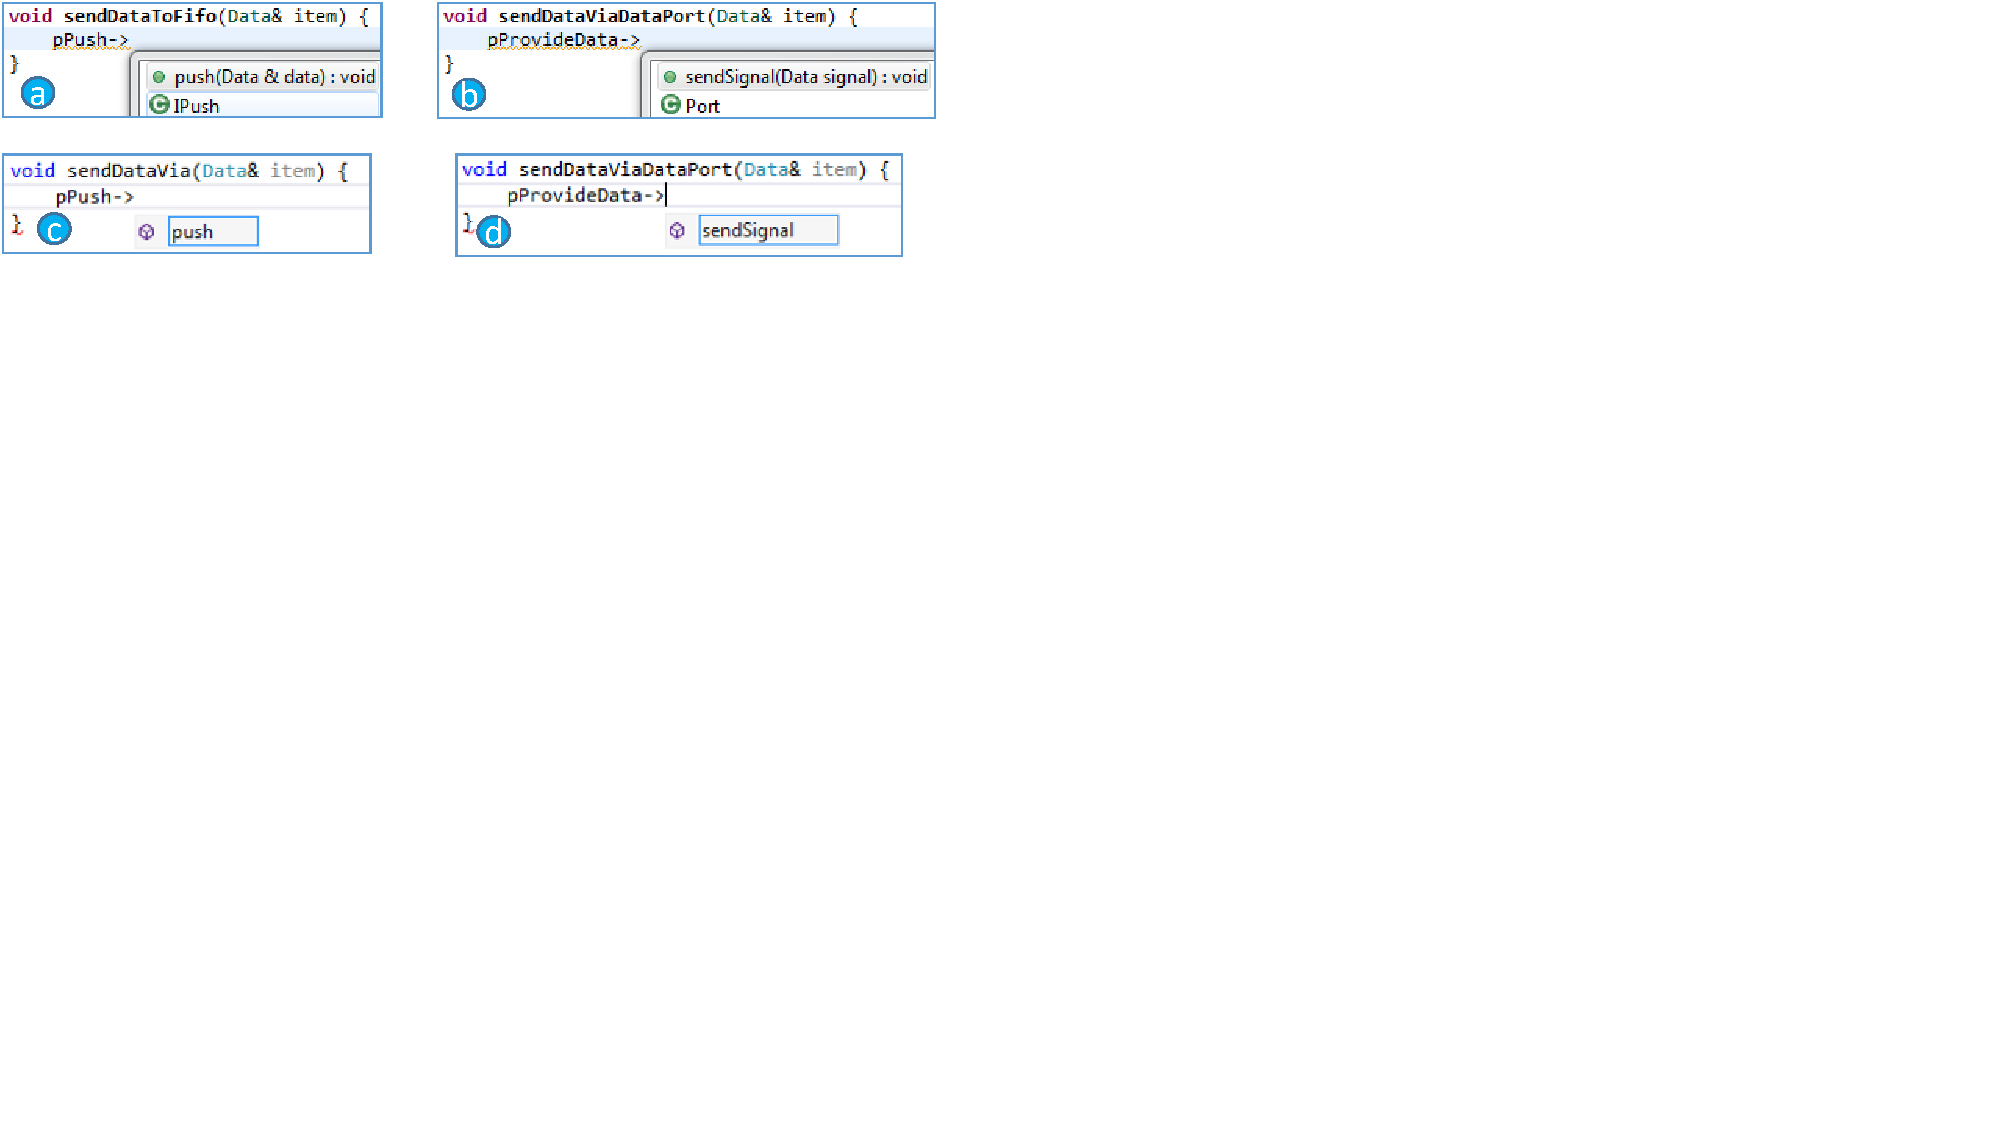
\includegraphics[clip, trim=0cm 14.6cm 17.7cm 0cm, width=\columnwidth]{figures/autocompletion.pdf}
	\caption{Auto-completions for XSeparation-generated code from the examples with interface and data ports: (a) and (b) in CDT and (c) and (d) in Visual Studio} 
	\label{fig:autocompletion}
\end{figure}
\end{comment}

After implementation, we then use the prototype with its use-cases to develop a software application for LEGO in order to evaluate XSeparation through the tooling prototype.
The followings present the case study development for the applicability evaluation and a manual evaluation of the usability.
%\subsection{Implementation}

Expressibility evaluation???

\subsection{Case study-based evaluation}

\subsubsection{Evaluation purpose}

\subsubsection{Case study development scenarios}

Description of the application...

The case study was developed by a developer \tb{Dev}. 
\tb{Dev} used the Papyrus Designer tool, which features component-based and model-driven development in UML and full C++ code generation through embedding of fine-grained code as blocks of texts within a limited text editor.   

During the development, an architecture model is created.
However, the developer felt difficult, unfamiliar, and annoyed to write code with the limited editor.
\tb{Dev} then refused to use that editor and programmed in CDT to be familiar and effective with C++ facilities such as syntax highlights and auto-completion.
\tb{Dev} then copied the code from CDT to the model and regenerated the code.
The developer felt inefficient, prone-to-error, and lack comprehension of the architecture information during code writing and copying.

Given the above issues, \tb{Dev} wants to try a synchronization approach, which at least can automatically synchronize modifications in fine-grained behavior to the model.

\vskip 0.1cm
\noindent
\tb{Application of XSeparation}:
Two developers: \tb{Dev} and another developer use Git to collaborate. 
Two distinct scenarios are emulated: (1) The developers modify both model and code; and (2) A collaboration scenario between \tb{Dev}, as a programmer, and the other as a software architect. 


\vskip 0.1cm
\noindent
\tb{Scenario 1}:
In this scenario, \tb{Dev} managed the application revision by using Git.
\tb{Dev} used Papyrus Designer to create the architecture model, and generates intermediate and executable code from it.
She then filled fine-grained behavior in the intermediate code using CDT.
After that, \tb{Dev} then used XSeparation to regenerate the executable code and compiled it.
The modified intermediate code is then automatically synchronized back to the original architecture model by using XSeparation.
Following each synchronization, \tb{Dev} committed and pushed both of the model, the intermediate code, and the executable code to Git.  

\vskip 0.1cm
\noindent
\tb{Scenario 2}:
\tb{Dev} and an other developer \tb{OtherDev} use Git to control versions of the case study project and work together.
In the beginning, the component-based architecture structure model is created by the two developers using Papyrus Designer.
Intermediate and executable code are then generated from the model by XSeparation.
The model and codes are then pushed to the Git repository as an initial version.
Each developer took in charge of development of several components.
For each corresponding component, each of the developers then described its course-grained behavior via a UML State machine, regenerated the intermediate code, wrote fine-grained code for the component, and synchronized the modified intermediate code with the model by using XSeparation.
After synchronization, the developer tried to pulled the artifacts from the remote Git repository.
If the remote model was updated by the other developer, both of the models were merged with each other using the Papyrus model merger \cite{collaborativepapyrus}.
After merging, the intermediate code is then regenerated.
The two artifacts are then pushed to the remote repository.
  


%\subsection{Evaluations of Incremental code generation and reverse engineering in XSeparation}

\subsection{Findings}
To evaluate the usability of XSeparation, several questions are used for asking developers for how effective XSeparation is when compared to full code generation approaches using fine-grained code directly embedded within models.

\paragraph{Is model-code synchronization in XSeparation better than full code generation with fine-grained code within models in general?}

\paragraph{Is modifying architecture at the code level more effective than at the model level?}

\paragraph{Is modifying fine-grained code at the code level better than code embedded within models for full code generation?}

\paragraph{Is concurrent development using XSeparation effective?}

\lipsum[1-2]
